%<dscrpt>Présentation ensembliste de la distance et d'un code de Hamming.</dscrpt>
L'objectif de ce problème est de présenter dans un cadre ensembliste la \emph{distance de Hamming} ainsi qu'un exemple de \emph{code de Hamming}\footnote{d'après \href{http://fr.wikipedia.org/wiki/Code\_de\_Hamming}{http://fr.wikipedia.org/wiki/Code\_de\_Hamming}}.\newline
Pour tout ensemble fini $E$, on notera $\sharp E$ son cardinal (nombre d'éléments).
\subsection*{Partie I. Différence symétrique.}
Dans cette partie $\Omega$ désigne un ensemble fini. Pour toute partie $X$ de $\Omega$, le complémentaire de $X$ dans $\Omega$ est noté $\overline{X}$ et la fonction caractéristique de $X$ est notée $1_X$.
\begin{displaymath}
\forall x \in \Omega, \;  1_X(x) =  
\left\lbrace 
\begin{aligned}
1& \text{ si } x \in X \\ 0& \text{ sinon }
\end{aligned}
\right. 
\end{displaymath}

On définit dans $\mathcal P(\Omega)$ une opération (notée $\Delta$) appelée \emph{différence symétrique} par :
\begin{displaymath}
 \forall (X,Y)\in \mathcal P(\Omega)\times \mathcal P(\Omega) :
X \mathop{\Delta} Y = (\overline{X}\cap Y)\cup(X \cap \overline{Y})
\end{displaymath}
\begin{enumerate}
 \item \begin{enumerate}
 \item Vérifier les propriétés suivantes et les traduire dans le vocabulaire des opérations:
\begin{align*}
(P1)& &\forall (X,Y)\in \mathcal P(\Omega)\times \mathcal P(\Omega) :& &X \mathop{\Delta} Y = Y \mathop{\Delta} X \\
(P2)& &\forall X \in \mathcal P(\Omega) :& &X \mathop{\Delta} \emptyset = \emptyset \mathop{\Delta} X = X\\
(P3)& &\forall X \in \mathcal P(\Omega) :& &X \mathop{\Delta} X = \emptyset 
\end{align*}
\item Montrer que :
\begin{displaymath}
\forall (X,Y)\in \mathcal P(\Omega)^2, \forall x\in \Omega,\hspace{0.5cm} x \in X \mathop{\Delta} Y \Leftrightarrow 1_X(x) + 1_Y(x) \equiv 1 \mod 2.  
\end{displaymath}

\end{enumerate}

\begin{figure}[ht]
 \centering
<<<<<<< HEAD
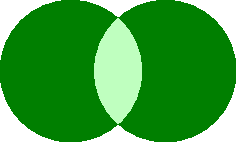
\includegraphics{./Ehamm_1.pdf}
\caption{Différence symétrique}
\label{fig:Ehamm_1}
=======
 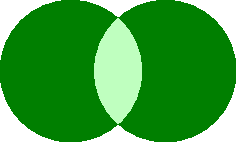
\includegraphics{./Ehamm_1.pdf}
 \caption{Différence symétrique}
 \label{fig:Ehamm_1}
>>>>>>> ee6f5760ebf9ef14a95501d6931d6c89435104c0
\end{figure}

\item \begin{enumerate}
 \item Montrer que 
\begin{displaymath}
 \forall (X,Y)\in \mathcal P(\Omega)\times \mathcal P(\Omega) :
\overline{X \mathop{\Delta} Y} = \left( \overline{X\cup Y}\right) \cup \left(X\cap Y \right)
\end{displaymath}
\item Soient $X$, $Y$, $Z$ trois parties de $\Omega$. Exprimer $X\mathop{\Delta}( Y\mathop{\Delta} Z)$ comme une union de parties deux à deux disjointes, chacune de ces parties étant une intersection de trois. En déduire l'associativité de $\mathop{\Delta}$.
\item Soient $X_1, X_2, \cdots ,X_p$ des parties de $\Omega$ et $x$ un élément de $\Omega$. Montrer que
\begin{displaymath}
 x \in X_1 \mathop{\Delta} \cdots \mathop{\Delta} X_p
 \Leftrightarrow 1_{X_1}(x) + \cdots + 1_{X_p}(x) \equiv 1 \mod 2.
\end{displaymath}
Comme $\mathop{\Delta}$ est associative, il est inutile d'écrire des parenthèses dans $X_1 \mathop{\Delta} \cdots \mathop{\Delta} X_p$.
\end{enumerate}

\item Dans cette question $A$, $B$, $C$ sont des parties quelconques de $\Omega$.
\begin{enumerate}
 \item Montrer que $A\mathop{\Delta} B \subset A \cup B$ et que :
\begin{displaymath}
 A\mathop{\Delta} B = \emptyset \Rightarrow A=B
\end{displaymath}
\item Simplifier $\left(A\mathop{\Delta} C \right)\mathop{\Delta} \left(C\mathop{\Delta} B \right)$ et $A\mathop{\Delta}\left( \left(A\mathop{\Delta} C \right)\mathop{\Delta} \left(C\mathop{\Delta} B \right)\right)$.
\end{enumerate}
\item Pour tout élément $u\in \Omega$ et toute partie $X$ de $\Omega$, on note $X_u = \{u\}\mathop{\Delta} X$. \begin{enumerate}
\item  Préciser $X_u$.
\item Soit $B$ une partie quelconque de $\Omega$. Montrer que :
\begin{displaymath}
\sharp(X_u\cap B) \equiv 
\left\lbrace 
\begin{aligned}
 &\sharp(X\cap B) +1 \text{ si }& u\in B \\
 &\sharp(X\cap B)  \text{ si }& u\notin B
\end{aligned}
\right. 
\mod 2.
\end{displaymath}
\end{enumerate}

\item Ici $\Omega$ contient $n$ éléments. Pour tout $A \subset \Omega$, on désigne par $\mathcal P_A$ l'ensemble des parties $X$ de $\Omega$ telles que 
\begin{displaymath}
 \sharp(X\cap A) \equiv 0 \mod 2
\end{displaymath}
\begin{enumerate}
 \item Montrer que $\sharp \mathcal P_A = 2^{n-1}$ lorsque $A$ est non vide.
\item Soient $A_1$ et $A_2$ deux parties non vides et distinctes de $\Omega$. Montrer que
\begin{displaymath}
 \sharp \left( \mathcal P_{A_1}\cap \mathcal P_{A_2}\right) = 2^{n-2}
\end{displaymath}
\item Soient $A_1$ et $A_2$ $A_3$ trois parties non vides, deux à deux distinctes de $\Omega$. On suppose de plus que $A_3$ n'est pas incluse dans $A_1\cup A_2$. Montrer que
\begin{displaymath}
 \sharp \left( \mathcal P_{A_1}\cap \mathcal P_{A_2} \cap \mathcal P_{A_3}\right) = 2^{n-3}
\end{displaymath}
\end{enumerate}
\end{enumerate}

\subsection*{Partie II. Distance de Hamming.}
On reprend les notations de la section précédente et on définit la \emph{distance de Hamming} $d(X,Y)$ entre deux parties $X$ et $Y$ de $\Omega$ par
\begin{displaymath}
\forall (X,Y)\in \mathcal P(\Omega)\times \mathcal P(\Omega) :
d(X,Y)= \sharp (X\mathop{\Delta} Y).
\end{displaymath}
\begin{enumerate}
 \item Montrer que  $d(A,B)=0$ entraîne $A=B$ pour toutes parties $A$ et $B$ de $\Omega$.

 \item Montrer l'inégalité triangulaire :
\begin{displaymath}
 \forall(A,B,C)\in\left( \mathcal P(\Omega)\right)^3 : 
d(A,B) \leq d(A,C) + d(C,B) 
\end{displaymath}

  \item Soit $C \subset \Omega$ et $k \in  \N$, on définit la \emph{H-sphère} de centre $C$ et de rayon $k$ (notée $\mathcal S(C,k)$) et la \emph{H-boule} de centre $C$ et de rayon $k$ (notée $\mathcal B(C,k)$) par :
\begin{displaymath}
 \forall X \in \mathcal P(\Omega), \hspace{0.5cm}
\left\lbrace 
\begin{aligned}
X\in \mathcal S(C,k) &\Leftrightarrow& d(C,X) = k \\
X\in \mathcal B(C,k) &\Leftrightarrow& d(C,X) \leq k  
\end{aligned}
\right. 
\end{displaymath}
On note $n$ le nombre d'éléments de $\Omega$. Quel est le nombre d'éléments d'une sphère de rayon $k$ ? Quel est le nombre d'éléments d'une boule de rayon $k$ ?  
\end{enumerate}

\subsection*{Partie III. Communiquer sûrement c'est organiser le délayage.}
Dans cette partie $E$ désigne un ensemble à $p$ éléments. On imagine un système de transmission qui \og émet\fg~ des parties $X$ de $E$ vers un récepteur. Mais de petites erreurs peuvent survenir lors de la transmission et de temps en temps le $X$ reçu n'est pas tout à fait le $X$ émis. Pour remédier à cela, on va transformer (coder) le $X$ en $\Phi(X)$ de sorte que chaque $\Phi(X)$ soit \og isolé\fg~ puis transmettre le $\Phi(X)$. Si une petite erreur survient lors de la transmission, le récepteur saura la repérer et éventuellement la corriger ou demander une nouvelle émission. Il devra ensuite décoder le $\phi(X)$ en $X$.\\
On suppose donc l'existence d'un ensemble $F$ à $n$ éléments contenant $E$, de $k\in \N$ et d'une application $\Phi$ de $\mathcal P(E)$ dans $\mathcal P(F)$ telle que :
\begin{displaymath}
 \forall (X,Y)\in \mathcal P(E), \hspace{0.5cm} X \neq Y
\Rightarrow d(\Phi(X),\Phi(Y)) > k
\end{displaymath}
où $d$ désigne la distance de Hamming dans $\mathcal P(F)$.

\begin{enumerate}
 \item Que signifie pour $\Phi$ le fait que $k$ soit supérieur ou égal à $0$ ?
 
 \item On suppose $k$ non nul et pair. Montrer que :
\begin{displaymath}
\forall (X,Y) \in \mathcal{P}(E)^2, \hspace{0.5cm} X \neq Y \Rightarrow \mathcal B(\Phi(X),\frac{k}{2}) \cap \mathcal B(\Phi(Y),\frac{k}{2}) = \emptyset
\end{displaymath}

  \item \begin{enumerate}
\item On suppose $k=2$. Montrer que $n+1\leq 2^{n-p}$. Quelle est la plus petite valeur possible pour $n$ si $p=4$?
\item  On suppose $k=4$. Former une inégalité que doivent vérifier $p$ et $n$. Quelle est la plus petite valeur possible pour $n$ si $p=4$ ?
\end{enumerate}

\end{enumerate}

\subsection*{Partie IV. Code de Hamming.}
L'objet de cette section est de donner un exemple de fonction $\Phi$ vérifiant les propriétés de la section III. Ici, $E$ est un ensemble à $4$ éléments et $F$ est un ensemble à $7$ éléments contenant $E$. On note
\begin{displaymath}
 E = \left\lbrace d_1,d_2,d_3,d_4\right\rbrace \hspace{1cm} F= \left\lbrace d_1,d_2,d_3,d_4,p_1,p_2,p_3\right\rbrace 
\end{displaymath}
Certaines parties de $F$, notées $A_1$, $A_2$, $A_3$, vont jouer un rôle particulier :
\begin{displaymath}
A_1 = \left\lbrace d_1,d_2,d_4,p_1\right\rbrace \hspace{1cm}
A_2 = \left\lbrace d_1,d_3,d_4,p_2\right\rbrace \hspace{1cm}
A_3 = \left\lbrace d_2,d_3,d_4,p_3\right\rbrace \hspace{1cm}
\end{displaymath}

On définit une fonction $\phi$ de $\mathcal P(E)$ dans $\mathcal P(F)$ la manière suivante.
\begin{displaymath}
 \forall X\in \mathcal P(E), \Phi(X)\text{ défini par }:
\left\lbrace 
\begin{aligned}
 &\Phi(X) \cap E = X \\
&p_1\in \Phi(X) \Leftrightarrow \sharp\left(X\cap\{d_1,d_2,d_4\} \right) \text{ impair}\\
&p_2\in \Phi(X) \Leftrightarrow \sharp\left(X\cap\{d_1,d_3,d_4\} \right) \text{ impair}\\
&p_3\in \Phi(X) \Leftrightarrow \sharp\left(X\cap\{d_2,d_3,d_4\} \right) \text{ impair}\\ 
\end{aligned}
\right. 
\end{displaymath}
\begin{enumerate}
 \item Calculer $\Phi(\emptyset)$, $\Phi(E)$, $\Phi(\{d_1\})$, $\Phi(\{d_1,d_2,d_4\})$.
 \item Montrer que, pour toute partie $X$ de $E$ et tout entier $i$ entre 1 et 3, $A_i\cap \Phi(X)$ contient un nombre pair d'éléments.
\item Montrer que, pour toute partie non vide $Z$ de $F$ :
\begin{displaymath}
 \sharp Z \leq 2 \Rightarrow \exists i \in \{1,2,3\} \text{ tel que } \sharp\left(  A_i\cap Z\right)  =1
\end{displaymath}
\item Soient $A$, $U$, $V$ des parties quelconques de $F$, montrer que
\begin{displaymath}
 \sharp(A\cap U) - \sharp(A\cap V) \equiv \sharp\left(A\cap (U\mathop{\Delta} V) \right) \mod 2 
\end{displaymath}
\item Montrer que pour toutes parties (de $E$) $X$ et $Y$ distinctes , la distance de Hamming entre $\Phi(X)$ et $\Phi(Y)$ est strictement plus grande que $2$.
\item (hors barême)\footnote{pour aller plus loin, il est bien plus commode d'utiliser la présentation classique des codes correcteurs à base d'algèbre linéaire sur le corps à deux éléments} Soit $Z$ une partie de $F$. Montrer qu'il existe une partie $X$ de $E$ telle que $Z=\Phi(X)$ si et seulement si $\sharp(A_1\cap Z)$, $\sharp(A_2\cap Z)$, $\sharp(A_3\cap Z)$ sont pairs.
\end{enumerate}
